\documentclass{book}
\usepackage{amsmath}
\usepackage[most]{tcolorbox}
\usepackage{cleveref}
\usepackage{titlesec}
\usepackage{graphicx}

\graphicspath{ {./imagenes/} }

\titleformat{\chapter}[display]
  {\normalfont\bfseries}{}{0pt}{\Huge}

\tcbset{theostyle/.style={
    enhanced,
    sharp corners,
    attach boxed title to top left={
      xshift=-1mm,
      yshift=-4mm,
      yshifttext=-1mm
    },
    top=1.5ex,
    colback=white,
    colframe=black!75!black,
    fonttitle=\bfseries,
    boxed title style={
      sharp corners,
    size=small,
    colback=black!75!black,
    colframe=black!75!black,
  } 
}}

\newtcbtheorem[number within=chapter]{Definition}{Definición}{%
  theostyle
}{def}


\begin{document}

\chapter{Tipos de enlaces covalentes}

\begin{Definition}{}{ReadingTheManual}
  \textbf{Enlace covalente:} Enalce dado entre elementos no metálicos para formar \textbf{moléculas covalentes}. Los enlaces se forman ya que las moléculas \textbf{comparten} 
  electrónes para llegar a ser estables (\textit{cumplir la regla del octeto}).
\end{Definition}

\subsection{Enlaces sencillos, dobles, y tríples}

Vienen dados por el \textbf{número de electónes compartido}:

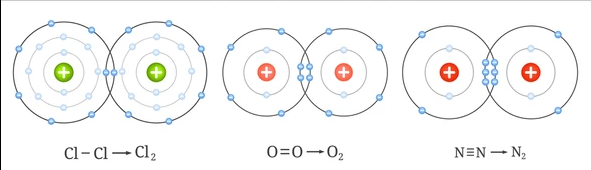
\includegraphics[scale=0.70]{enlaces-por-complejidad.png}

\section{Elementos covalentes}


\begin{tabular}{| c | c c |}
  \hline
  Estado de agregación & Ejemplos & Propiedades generales \\
  \hline
  Cristalino & 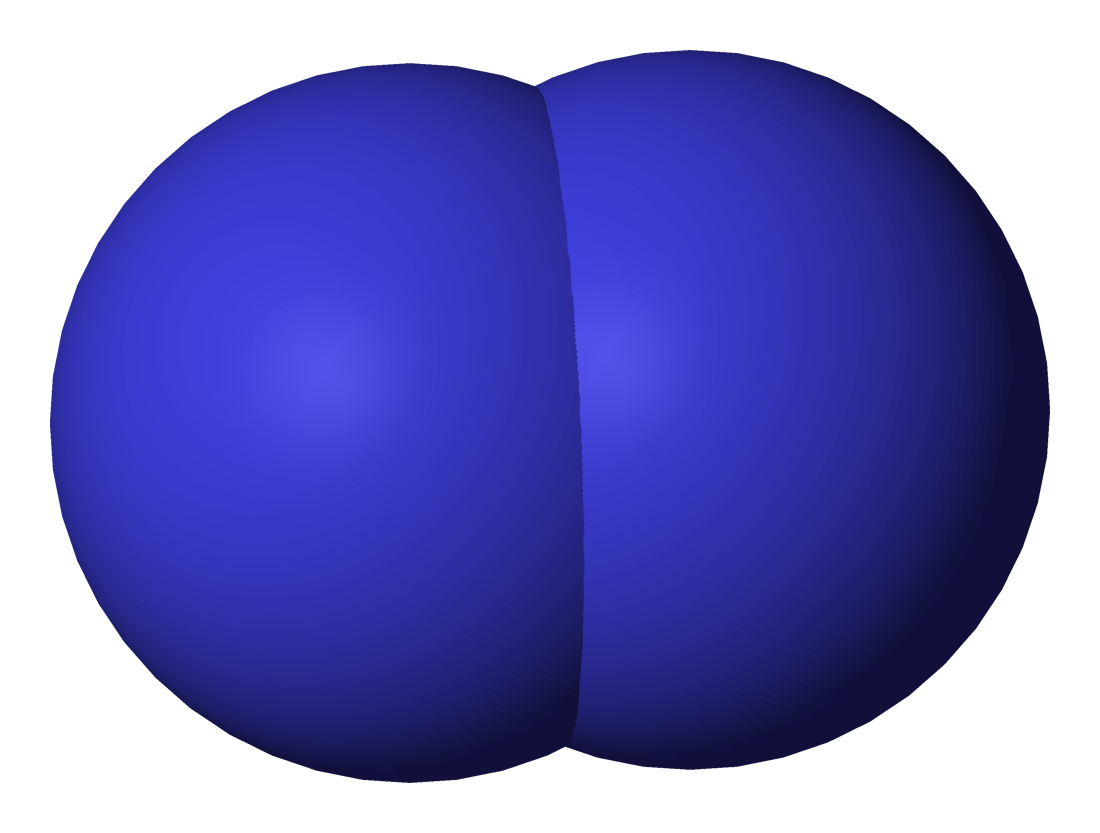
\includegraphics[scale=0.05]{dinitrogeno.png} \textit{$ N_{2} $} & s \\
  \hline
  Molecular & 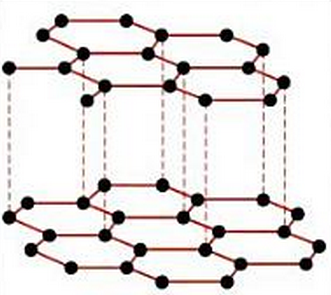
\includegraphics[scale=0.20]{grafito.png} \textit{$ C $} & 788 \\
  \hline
\end{tabular}

\section{Compuestos covalentes}

\begin{tabular}{| c | c c |}
  \hline
  Estado de agregación & Ejemplos & Propiedades generales \\
  \hline
  Cristalino & 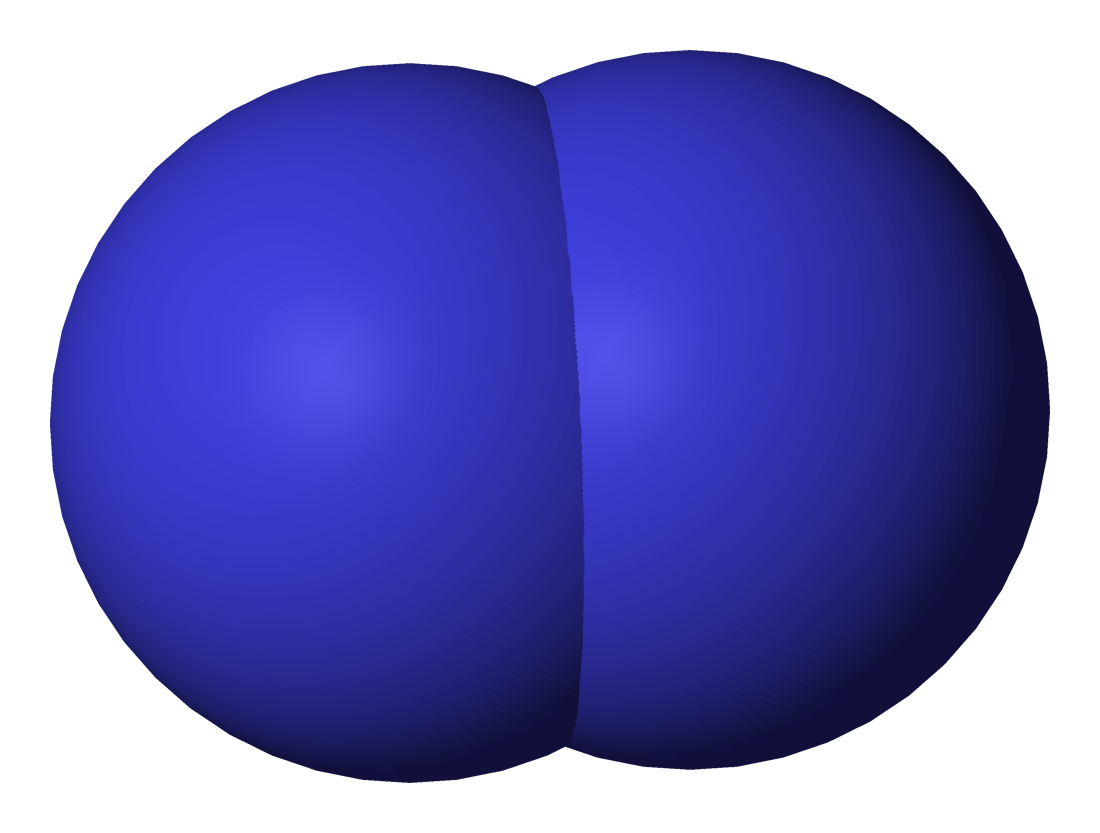
\includegraphics[scale=0.05]{dinitrogeno.png} \textit{$ N_{2} $} & s \\
  \hline
  Molecular & 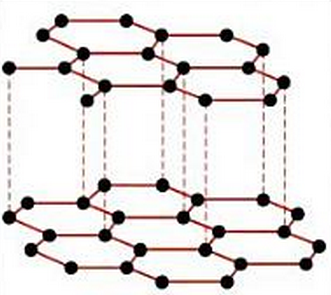
\includegraphics[scale=0.20]{grafito.png} \textit{$ C $} & 788 \\
  \hline
\end{tabular}


\end{document}